%!TEX root = ../dissertation.tex
%\begin{figure}
%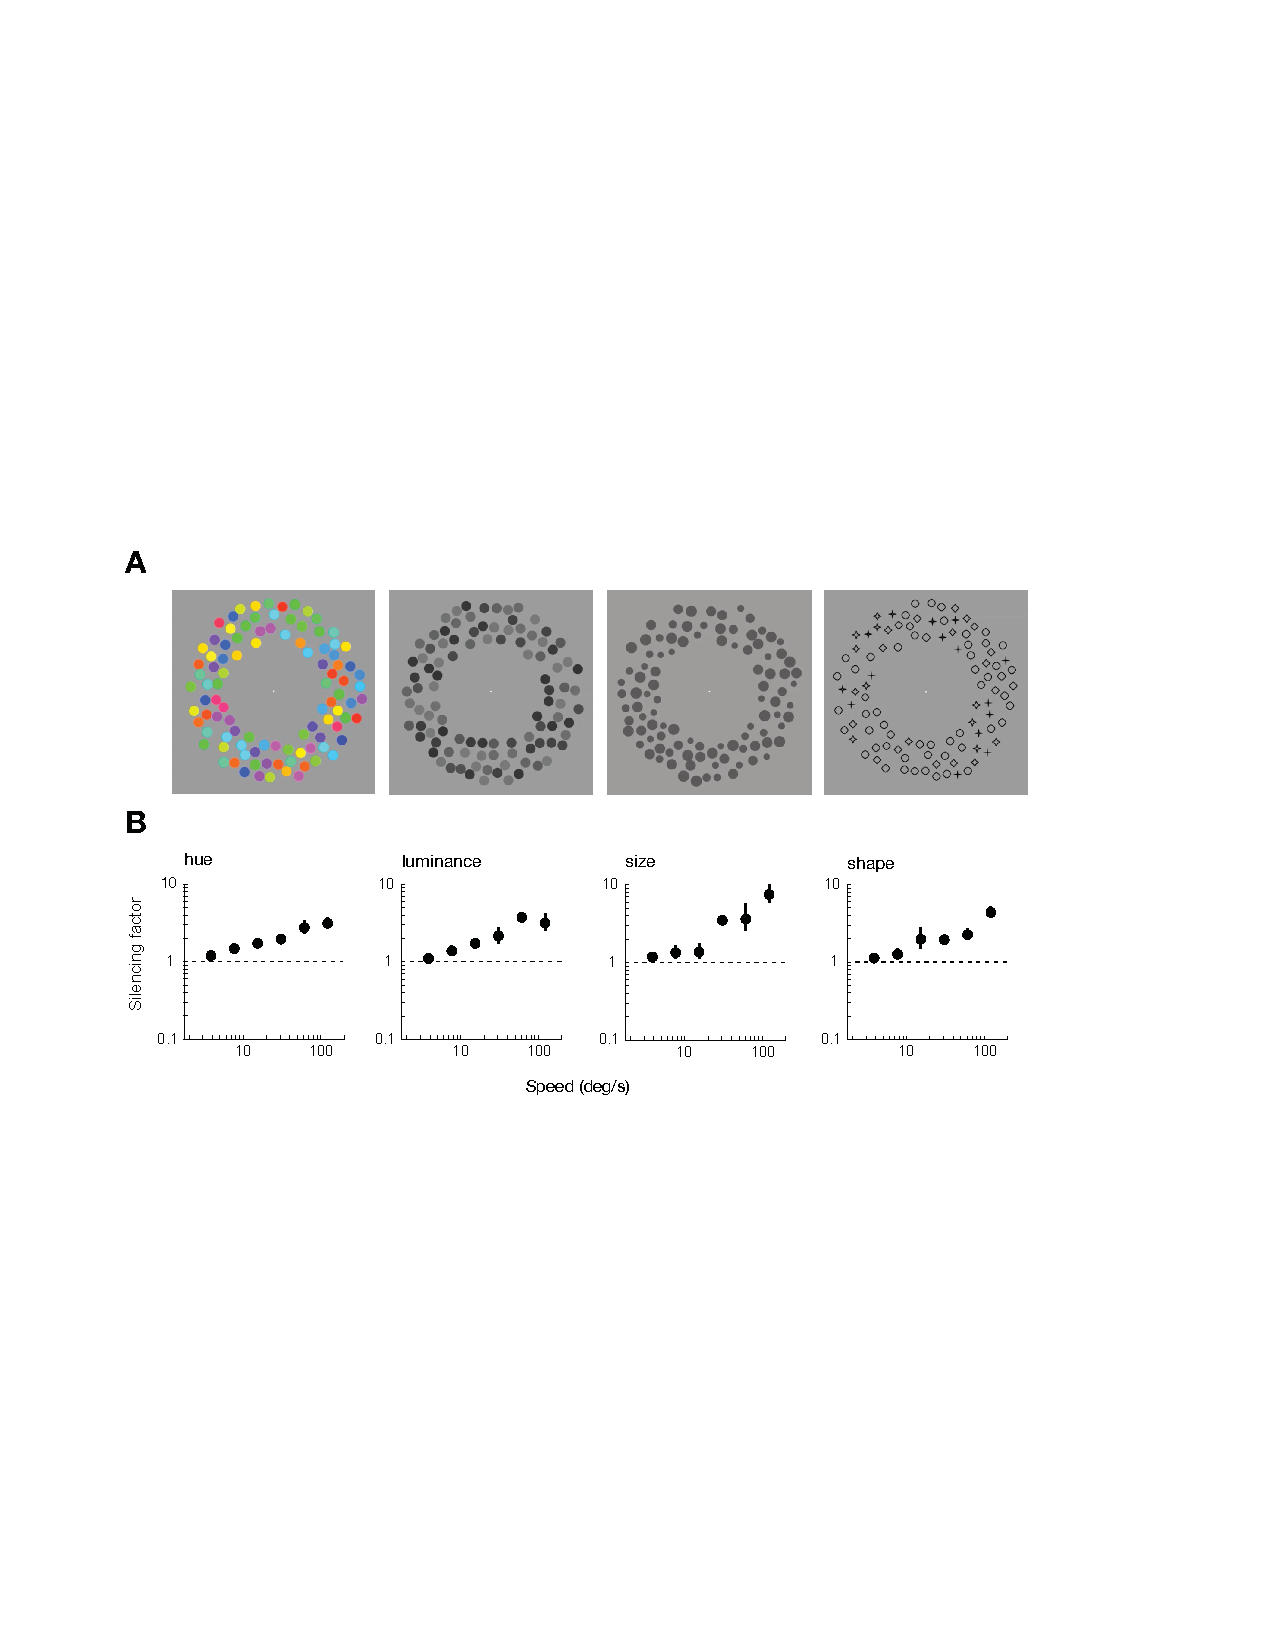
\includegraphics[width=\textwidth]{figures/fig1}
%\caption[Short figure name.]{This is a figure that floats inline and here is its caption.
%\label{fig:myInlineFigure}} \end{figure}

% For an example of a full page figure, see Fig.~\ref{fig:myFullPageFigure}.


% For an example of a full page figure, see Fig.~\ref{fig:myFullPageFigure}.
\chapter{Il progetto aziendale}
Il seguente capitolo illustra gli aspetti principali dello stage, il contesto di inserimento, gli obiettivi prefissati e le prospettive dell’azienda. Questo
permette di comprendere il ruolo che ricoprono i progetti di stage all’interno della strategia aziendale.
\section{Proposta di stage}
Pur essendo un’azienda che offre principalmente servizi di consulenza e assistenza, NETCOM presenta anche un reparto di Ricerca e Sviluppo, che si occupa dell'innovazione tecnologica e segue progetti per l’accrescimento dell’offerta fornita alla clientela.
L’azienda, tramite l'attività di stage offerta agli studenti laureandi, si  confronta con il mondo universitario e permette allo studente di acquisire competenze e applicare le proprie conoscenze all’attività lavorativa.
Da anni NETCOM partecipa all'evento \gl{Stage-IT} e presenta alcune possibili proposte di progetti in cui il laureando può essere inserito. 
Personalmente, dopo aver conosciuto l'azienda a Stage-IT, ho fissato un colloquio con l’azienda e discusso sulle possibili offerte di stage.
La proposta di stage offertami da NETCOM è stata quella di essere inserita all’interno del loro dipartimento Ricerca e Sviluppo per partecipare allo sviluppo di \emph{Beryllium}, una piattaforma sviluppata dall' azienda per monitorare l'utilizzo di \emph{software} aziendali.

\section{Progetto Beryllium}

\subsection{Contesto di inserimento}
Attualmente, un numero crescente di aziende, affida in \emph{outsourcing} a \emph{service provider} alcuni dei servizi utilizzati così da potersi concentrare maggiormente sugli obiettivi aziendali.
I \emph{service provider} che offrono \emph{software} Microsoft alle aziende, sono soggetti a un particolare programma di \emph{licensing} chiamato \emph{Service Provider Level Agreement} (SPLA).
Il programma Microsoft SPLA prevede che ogni \emph{service provider} paghi a Microsoft una quota mensile che dipende all'utilizzo effettivo del \emph{software} da parte dei vari clienti e pertanto, ogni mese, un \emph{service provider} ha la necessità di generare un \emph{report} con l'effettivo utilizzo del \emph{software} Microsoft da inoltrare ad un rivenditore di contratti SPLA.
La generazione di questi report è solitamente un'attività manuale svolta da personale tecnico specializzato. 
"Beryllium SPLA Manager" è sviluppato allo scopo di automatizzare la generazione di \emph{report} e di offriren ai \emph{service provider} uno strumento completo che consente di monitorare e gestire i contratti SPLA stipulati.
L'applicativo è composto principalmente da 3 macro-componenti:
\begin{itemize}
    \item \emph{Web Portal Interface}: il portale \emph{web} attraverso cui ogni \emph{service provider} può monitorare l'utilizzo del \emph{software} Microsoft di ogni suo cliente, gestire i contratti SPLA e generare i \emph{report} mensili;
    \item \emph{Core Engine}: questa componente è il cuore del sistema e contiene
    l'intelligenza in grado aggregare i dati grezzi per renderli fruibili all'utente finale tramite il portale \emph{web};;
    \item \emph{Data Collector}: agente installato sulle macchine virtuali e fisiche di ogni \emph{service provider} che si occupa di raccogliere, su base giornaliera, i dati grezzi di utilizzo.
\end{itemize}
     \begin{figure}[H]
        \centering
        \captionsetup{justification=centering,margin=2cm}
            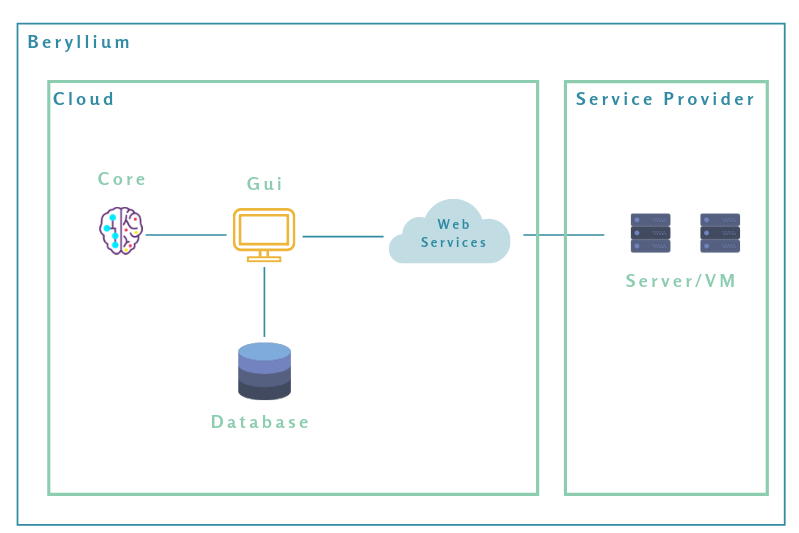
\includegraphics[width=0.6\textwidth ]{figures/Beryllium.png}
            \caption [Architettura macroscopica di Beryllium]{Architettura macroscopica di Beryllium \label{fig:Beryllium}}
    \end{figure}
\subsection{Progetto di stage}
Alla studentessa è stato richiesto di integrarsi con il team di sviluppo di NETCOM e collaborare con esso nella progettazione e implementazione di una soluzione per estrarre dati significativi per il \emph{licensing} dal prodotto \emph{Microsoft Dynamics} CRM 2016.
Il Data Collector (agente) è un servizio di Windows che in maniera schedulata
raccoglie tutti i dati grezzi che possono essere significativi per determinare il \emph{licensing} dei prodotti Microsoft supportati.
L'agente è stato progettato per essere modulare in modo tale che, per supportare un nuovo prodotto Microsoft, sia sufficiente aggiungere una \gl{DLL} in una cartella dell'agente.
Il progetto consiste nella realizzazione di una nuova \emph{feature} dell'agente (una nuova DLL) contenente le funzioni atte all'estrazione dei dati significativi per il \emph{licensing} del prodotto \emph{Microsoft Dynamics} CRM 2016.

Il progetto di stage offerto dall’azienda comprende tutte le attività che costituiscono il processo di sviluppo di un prodotto \emph{software}. Prima dell’inizio dello stage, il tutor Alessandro Strenghetto ha redatto un piano di lavoro per stabilire quali obiettivi dovessero essere raggiunti al suo termine. Relativamente al processo di sviluppo le attività previste dal progetto di stage sono:
\begin{itemize}
    \item Analisi dei requisiti;
    \item Progettazione;
    \item Codifica;
    \item Test;
    \item Verifica e Validazione.
\end{itemize}
Oltre alle attività sopra elencate, il piano include una prima fase di formazione necessaria all’apprendimento del funzionamento delle tecnologie e degli ambienti di sviluppo da utilizzare in modo da acquisire familiarità con gli strumenti che saranno impiegati nell’intero processo di sviluppo;
Inoltre è prevista una costante attività di documentazione, che deve accompagnare tutte le fasi del processo di sviluppo allo scopo di organizzare e tenere traccia di tutte le attività da svolgere durante lo stesso.\\
     \begin{figure}[H]
        \centering
        \captionsetup{justification=centering,margin=2cm}
            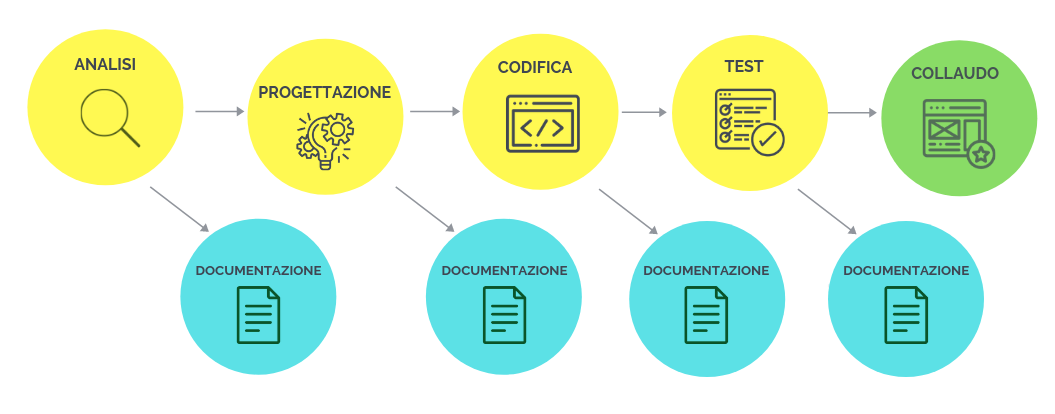
\includegraphics[width=0.8\textwidth ]{figures/pianolavoro.png}
            \caption [Obiettivi e metodo di lavoro NETCOM]{Obiettivi e metodo di lavoro proposto da NETCOM \label{fig:pianolavoro}}
    \end{figure}
\section{Vincoli}
Nel Piano di Lavoro, sono stati introdotti dei vincoli, sia di tipo lavorativo, sia di tipo tecnologico. 
Di seguito sono riportati i vincoli suddivisi per tipologia:
\begin{itemize}
    \item Vincoli lavorativi: questa categoria comprende i prodotti attesi al termine dello stage e le limitazioni imposte riguardanti la modalità di lavoro. Prima dell’inizio dell’attività di stage, con il tutor aziendale, sono stati stabiliti i seguenti prodotti attesi:
    \begin{itemize}
        \item Prototipo della componente "Microsoft Dynamics CRM
        feature for Beryllium Data Collector" per l’ultima versione di \emph{Microsoft Dynamics} CRM;
        \item Documentazione di progetto composta dai documenti Analisi dei Requisiti e Specifica Tecnica.
        \end{itemize}
Il tutor aziendale ha condiviso un modello per la documentazione, così da permettere l'allineamento con gli standard utilizzati in azienda ed avere una traccia nello sviluppo dei documenti. Per lo sviluppo è stato reso disponibile il codice dell’applicativo da integrare, in modo da poter acquisire familiarità con il prodotto, e successivamente il personale del dipartimento DEV mi ha guidata nella realizzazione dello stesso.

\item Vincoli tecnologici: questa categoria rappresenta tutte le condizioni e i limiti sulla tipologia di tecnologie da utilizzare per sviluppare i prodotti.
I vincoli imposti sono stati:
\begin{itemize}
    \item La \emph{feature Microsoft Dynamics} CRM deve essere compilabile con .NET framework 4.0. Eventuali librerie esterne utilizzate devono essere compatibili con .NET framework 4.0;
    \item La soluzione non deve richiedere l’installazione di \emph{tool} aggiuntivi sul \emph{server} del cliente;
    \item La soluzione deve essere retrocompatibile con la maggior parte delle versioni di \emph{Microsoft Dynamics} CRM;
    \item Il linguaggio con cui sviluppare la \emph{feature} è il C\#, con la possibilità di integrare del codice \emph{PowerShell} all’interno del codice in C\#;
    \item La \emph{feature} deve essere realizzata come libreria con estensione \emph{.dll};
    \item La codifica della \emph{feature} seguire la struttura decisa dall’azienda per potersi interfacciare con le altre componenti della piattaforma.
\end{itemize}
Ogni vincolo imposto è stato controllato dal tutor aziendale durante lo svolgimento dello stage.

\end{itemize}
\section{Piano di Lavoro}
Durante la fase di pianificazione dello stage è stato redatto un piano di lavoro in collaborazione con il tutor aziendale.
Allo scopo di delineare le attività da svolgere durante il corso dello stage, è stato prodotto un diagramma di Gantt, in cui è stata attribuita una certa quantità di ore che rappresenta la loro durata in termini orari di ogni attività. 
La durata delle attività è stata calcolata in modo da poter completare le stesse entro le 320 ore previste per lo stage formativo.
Tale pianificazione ha consentito alla studentessa e al tutor aziendale di avere una visione completa delle attività da svolgere e delle tempistiche a disposizione. \\
Il piano di lavoro non è stato modificato nel corso dello stage al fine di poter effettuare un bilancio al termine di esso.
\subsection{Obiettivi pianificati}
Attraverso la pianificazione del lavoro sono stati stabiliti gli obiettivi da raggiungere alla conclusione dello stage. 
Tutte le attività sono state ripartite in tre tipologie tipologie di obiettivi, a seconda della loro priorità. 
In particolare si fa riferimento ai requisiti secondo le seguenti notazioni:
\begin{itemize}
    \item O per i requisiti obbligatori, vincolanti in quanto obiettivo primario richiesto dal committente;
    \item D per i requisiti desiderabili, non vincolanti o strettamente necessari, ma dal riconoscibile valore aggiunto;
    \item F per i requisiti facoltativi, rappresentanti valore aggiunto non strettamente competitivo.
\end{itemize}
Tale suddivisione ha permesso di quantificare il lavoro svolto durante lo stage. 
Alle sigle precedentemente indicate è stata aggiunta una coppia sequenziale di numeri, creando l’identificativo finale del requisito.
Secondo la classificazione appena descritta gli obiettivi individuati con il tutor aziendale sono:
\begin{itemize}
    \item Obbligatori:
    \begin{itemize}
        \item O01: Studio dell’intero sistema \emph{Beryllium};
        \item O02: Comprensione del mondo SAM, SPLA e del prodotti Microsoft di interesse;
        \item O03: Configurazione dell’ambiente di test per il prodotto Microsoft Dynamics CRM;
        \item O04: Progettazione, sviluppo e test di un prototipo della componente "Microsoft Dynamics CRM feature for Beryllium Data Collector" per l’ultima versione di \emph{Microsoft Dynamics} CRM;
        \item O05: Documentazione di progetto.
    \end{itemize}
    \item Desiderabili:
    \begin{itemize}
        \item D01: Completa integrazione con la componente \emph{Beryllium Data Collector}.
    \end{itemize}
    \item Facoltativi:
    \begin{itemize}
        \item F01: Sviluppo e test della componente "Microsoft Dynamics CRM feature for Beryllium Data Collector" per almeno una versione più vecchia di \emph{Microsoft Dynamics} CRM;
        \item F02: Sviluppo e test della componente "Microsoft Dynamics CRM feature for Beryllium Data Collector" per almeno due versioni più vecchie di \emph{Microsoft Dynamics} CRM.
    \end{itemize}
\end{itemize}
\subsection{Pianificazione attività e scadenze}
Per raggiungere gli obiettivi prefissati sono state individuate una serie di attività che possono essere raggruppate in tre attività più estese:
\begin{itemize}
    \item Introduzione: rappresenta la fase iniziale del progetto dedicata alla formazione e all'inserimento della studentessa nel contesto aziendale. In particolare:
        \begin{itemize}
            \item Introduzione alle modalità di lavoro nel team di sviluppo: durante questa attività è prevista la descrizione delle fondamentali norme seguite dal team di Sviluppo, con particolare attenzione alla comprensione degli strumenti di versionamento utilizzati dall'azienda;
            \item Formazione sul sistema aziendale di infrastruttura virtuale: l'attività prevede l'apprendimento dell’utilizzo del sistema di virtualizzazione aziendale;
            \item Introduzione al progetto \emph{Beryllium}: durante questa attività viene presentato il progetto di lavoro, rivolgendo particolare attenzione a come le componenti sviluppate dalla studentessa andranno ad interfacciarsi con il resto del prodotto.
        \end{itemize}
    \item Analisi: rappresenta la prima attività del processo di sviluppo.
    In particolare:
        \begin{itemize}
            \item Analisi dell’intero sistema \emph{Beryllium}: attività in cui viene studiato il sistema esistente in modo da poter avere un’idea di massima sulla componente da realizzare durante lo stage;
            \item Analisi del \emph{data collector} di \emph{Beryllium}: attività in cui viene studiato l'agente installato sulle macchine virtuali e fisiche di ogni \emph{service provider};
            \item Analisi delle \emph{features} già esistenti del \emph{data collector} di \emph{Beryllium}: attività in cui vengono analizzate le \emph{features} precedentemente sviluppate ed integrate al fine di apprenderne la struttura e le funzionalità; 
            \item Identificazione requisiti: attività in cui vengono stabiliti i requisiti funzionali, di vincolo e di qualità del prodotto da sviluppare;
            \item Documentazione: stesura del documento di Analisi dei Requisiti per tenere traccia del lavoro di analisi svolto.
        \end{itemize}

    \item Progettazione: rappresenta l'attività che consiste nella determinazione dell’architettura del prodotto. 
    In particolare:
        \begin{itemize}
            \item Definizione architettura ad alto livello: attività che prevede la definizione della struttura della e la scelta dei \emph{design patterns};
            \item Definizione e organizzazione componenti: attività che corrisponde alla progettazione di dettaglio, in cui vengono individuate le classi del programma, i relativi metodi e l'interazione tra esse;
               \item Configurazione ambiente di test con \emph{Microsoft Dynamics} CRM: l'attività prevede la creazione e la configurazione dell'ambiente di test e l'installazione di strumenti utili allo stage;
            \item Documentazione: attività che consiste nella redazione del documento di Specifica Tecnica.
        \end{itemize}
    \item Codifica: rappresenta l'attività che consiste nell'implementazione della soluzione individuata. In particolare:
        \begin{itemize}
            \item Implementazione delle soluzioni individuate: attività che consiste nella realizzazione di ciò che è stato definito durante la progettazione;
            \item Documentazione: attività che consiste nella redazione della documentazione della \emph{feature Microsoft Dynamics} CRM
            con l’aggiunta di commenti in lingua inglese al codice prodotto.
        \end{itemize}
                        \clearpage
    \item Test: rappresenta l'attività di verifica prevista.
        \begin{itemize}
            \item \emph{Bug fix} e collaudo finale: attività che consiste nell'esecuzione di test delle diverse funzionalità dell'applicazione e della sua integrazione con il resto del progetto;
            \item Tracciamento dei requisiti: attività di validazione  permette di riconoscere quali requisiti sono stati soddisfatti.
        \end{itemize}
\end{itemize}
 \begin{figure}[H]
    \centering
    \captionsetup{justification=centering,margin=2cm}
        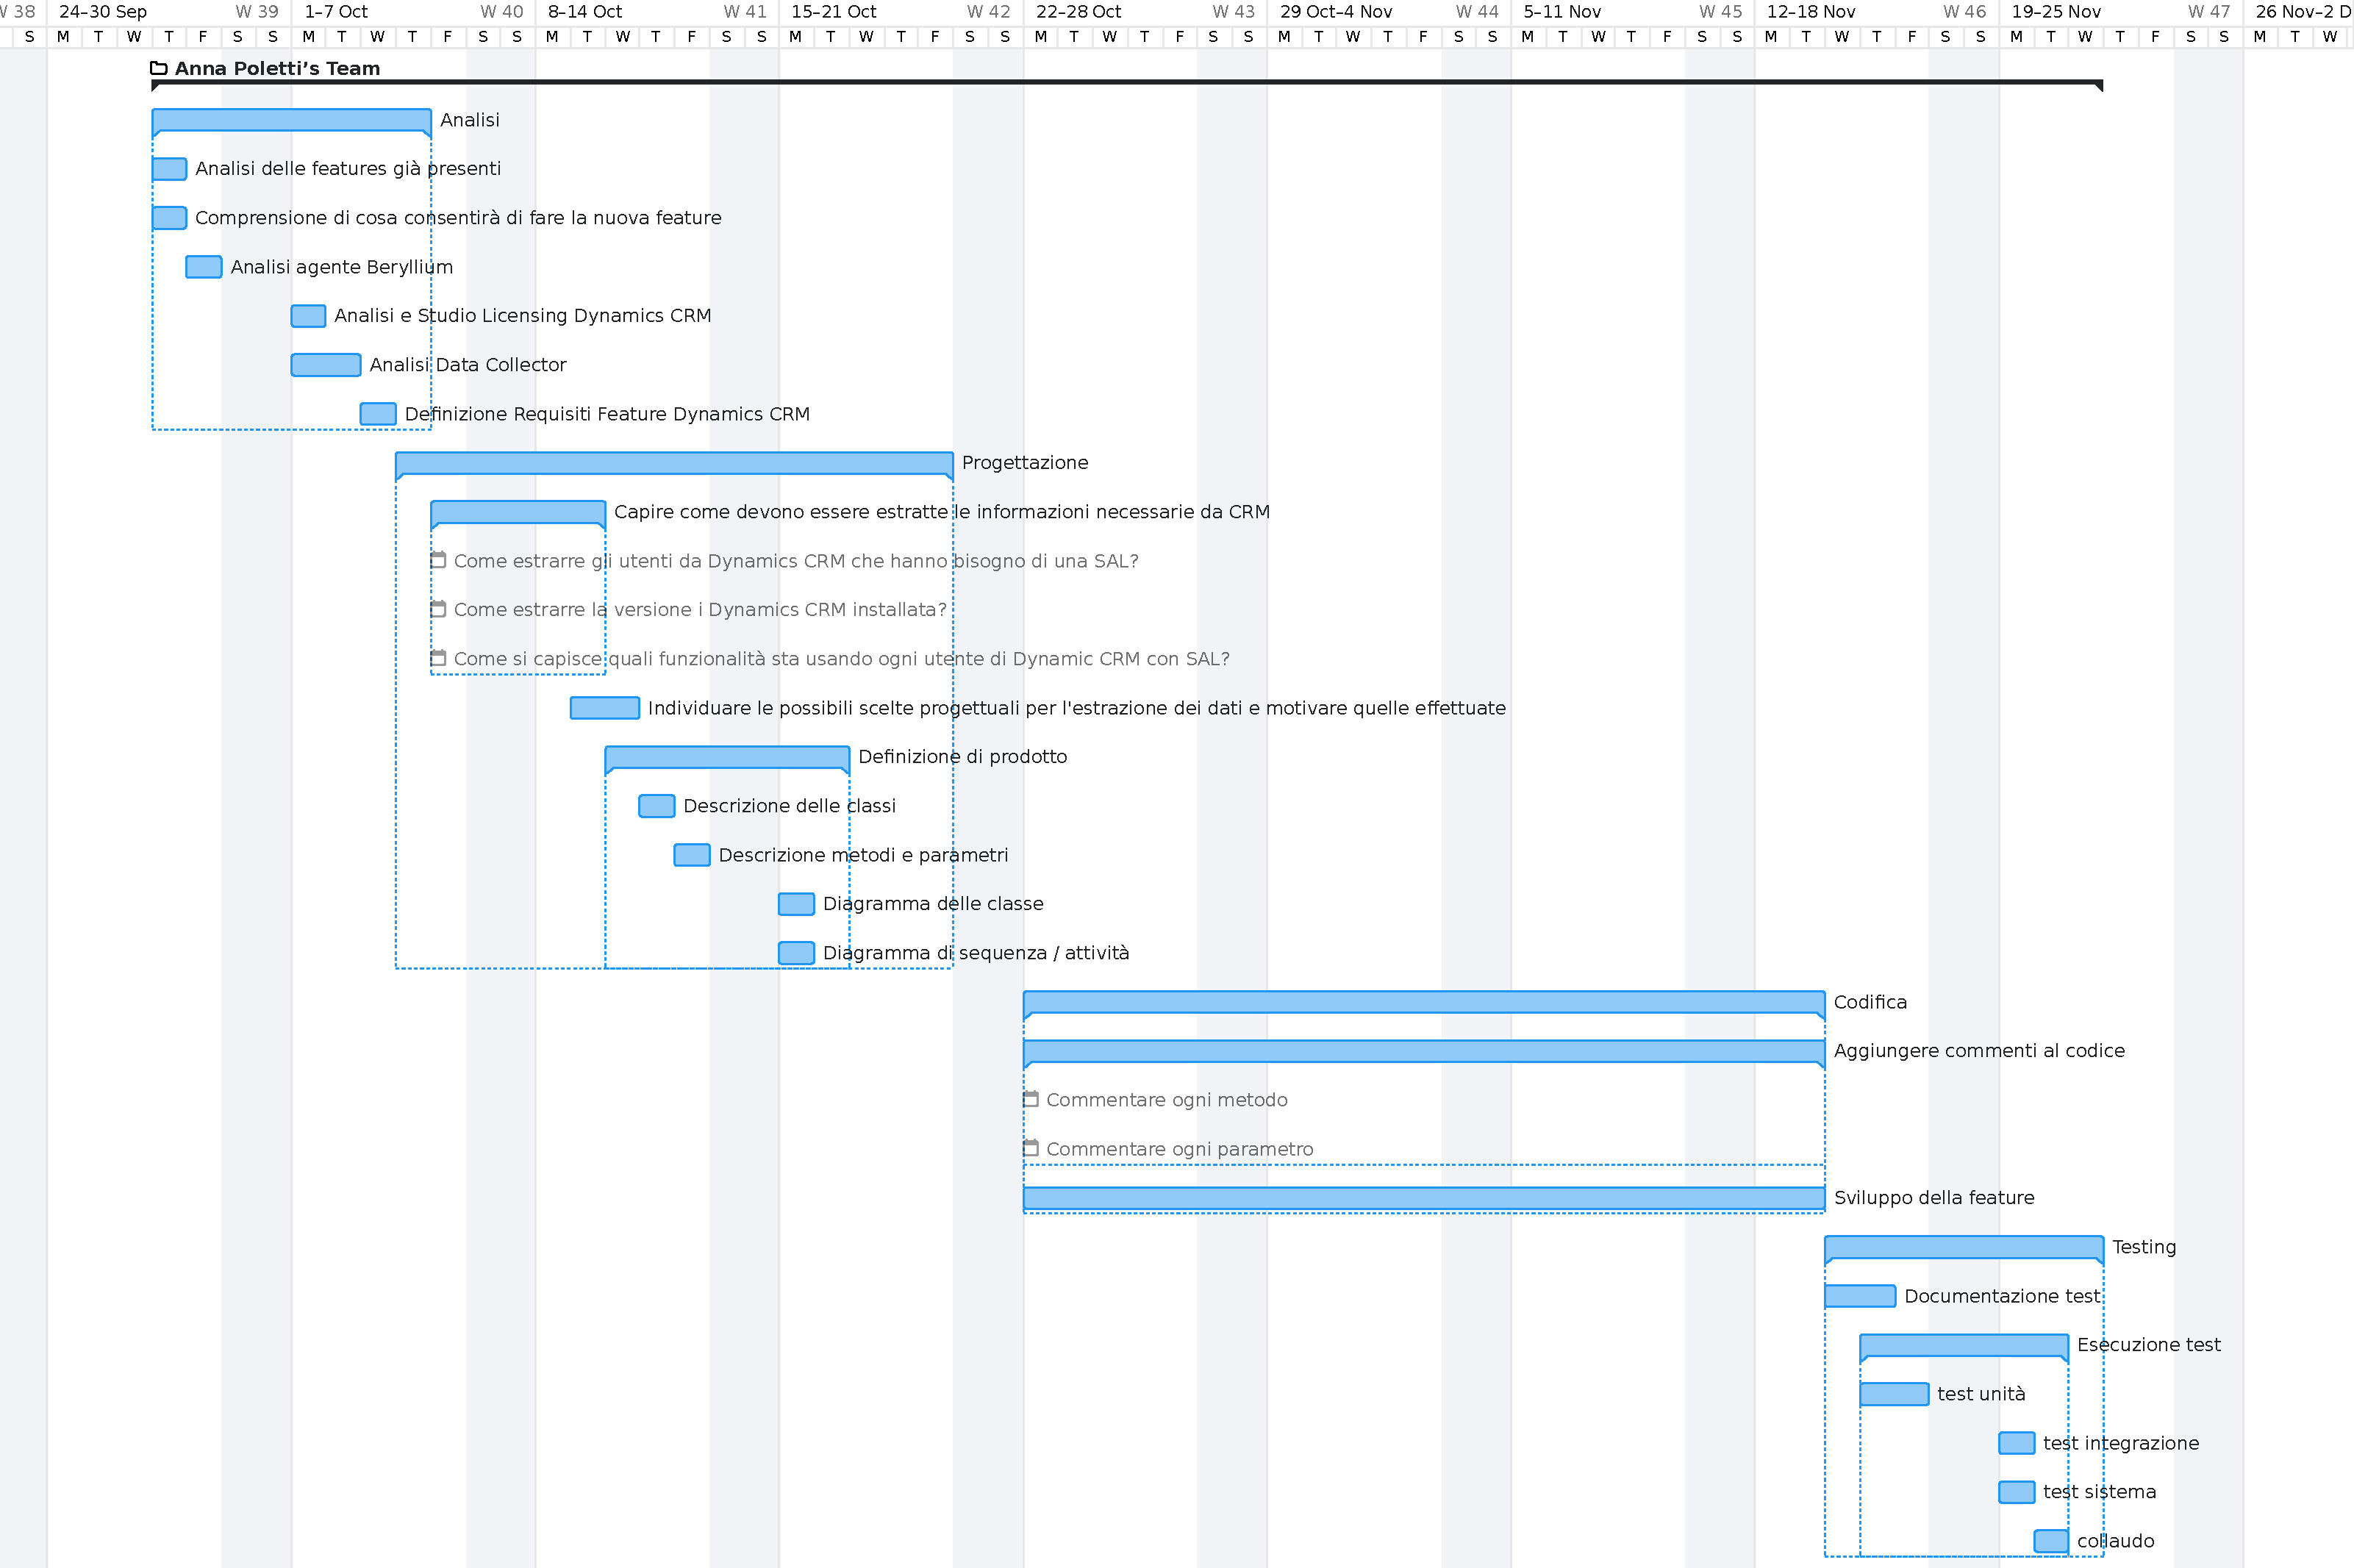
\includegraphics[width=0.8\textwidth ]{figures/gantt.pdf}
        \caption [Diagramma di Gantt: attività pianificate]{Diagramma di Gantt: dall'Analisi al Collaudo \label{fig:gantt}}
\end{figure}


%% Requires fltpage2 package
%%
% \begin{FPfigure}
% 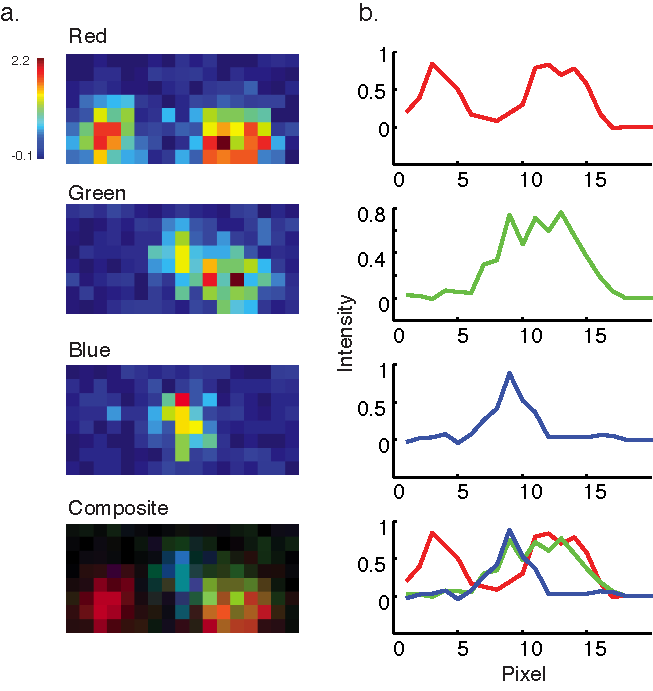
\includegraphics[width=\textwidth]{figures/fullpage}
% \caption[Short figure name.]{This is a full page figure using the FPfigure command. It takes up the whole page and the caption appears on the preceding page. Its useful for large figures. Harvard's rules about full page figures are tricky, but you don't have to worry about it because we took care of it for you. For example, the full figure is supposed to have a title in the same style as the caption but without the actual caption. The caption is supposed to appear alone on the preceding page with no other text. You do't have to worry about any of that. We have modified the fltpage package to make it work. This is a lengthy caption and it clearly would not fit on the same page as the figure. Note that you should only use the FPfigure command in instances where the figure really is too large. If the figure is small enough to fit by the caption than it does not produce the desired effect. Good luck with your thesis. I have to keep writing this to make the caption really long. LaTex is a lot of fun. You will enjoy working with it. Good luck on your post doctoral life! I am looking forward to mine. \label{fig:myFullPageFigure}}
% \end{FPfigure}
% \afterpage{\clearpage}
